% 请确保文件编码为utf-8,使用XeLaTex进行编译,或者通过overleaf进行编译

\documentclass[answers]{exam}  % 使用此行带有作答模块
% \documentclass{exam} % 使用此行只显示题目

\usepackage{xeCJK}
\usepackage{zhnumber}
\usepackage{graphicx}
\usepackage{hyperref}
\usepackage{amsmath}
\usepackage{booktabs}
\usepackage{enumerate}
\usepackage{amssymb}
\usepackage{bm}

\pagestyle{headandfoot}
\firstpageheadrule
\firstpageheader{南京大学}{高级机器学习}{习题集二}
\runningheader{南京大学}
{高级机器学习}
{习题集二}
\runningheadrule
\firstpagefooter{}{第\thepage\ 页(共\numpages 页)}{}
\runningfooter{}{第\thepage\ 页(共\numpages 页)}{}

% no box for solutions
% \unframedsolutions

\setlength\linefillheight{.5in}

% \renewcommand{\solutiontitle}{\noindent\textbf{答:}}
\renewcommand{\solutiontitle}{\noindent\textbf{解:}\par\noindent}

\renewcommand{\thequestion}{\zhnum{question}}
\renewcommand{\questionlabel}{\thequestion .}
\renewcommand{\thepartno}{\arabic{partno}}
\renewcommand{\partlabel}{\thepartno .}


\begin{document}
\Large

\begin{questions}
\question [30] \textbf{半监督学习}

关于半监督学习,课堂上介绍了为什么需要半监督学习以及半监督学习的几种基本做法。在前沿研究中,无论是计算机视觉还是自然语言处理领域,半监督学习仍然是研究重点。下面三个问题分别针对传统半监督学习、深度半监督学习进行拓展介绍。

\begin{parts}
	\part [10] 在TSVM中会对未标记的样本进行标记指派,这个本质上也是一种伪标签的应用。伪标签的含义就是给无标记数据赋予标签,最初这些标签可能绝大多数是错误的,但是会有一些是准确的,将这些准确的筛选出来加入有标记数据训练即可起到扩充训练集的效果。这也是TSVM的主要思想。因此,使用一个预训练模型给未标记数据打标签之后,该怎么做才能尽可能选出那些准确的样本呢?请提供至少三种启发式解决方案并说明理由。(提示:从置信度等角度出发)。试查阅主动学习(Active Learning)相关资料,介绍主动学习并分析其与基于伪标签半监督学习的区别。
	
	\part [10] 标记传播(Label Propagation)是一种非常有效的图半监督学习算法,将样本看做图的顶点,然后将标记从有标记样本扩散到未标记样本。该过程类似于PageRank算法,试描述PageRank算法并比较其与Label Propagation的区别。其余相关的算法还包括:Query Diffusion (QD)等。QD算法先计算样本点之间相似度$a_{ij}=s(x_i,x_j) \geq 0, \forall i, j \in [n]^2$(假设该相似度对称,即$a_{ij}=a_{ji}$),构成亲和矩阵(Affinity Matrix) $A\in \mathcal{R}^{(n+m)\times (n+m)}$,然后对每个样本点计算近邻集合$NN_k(i)$,$k$代表近邻样本数目,记$D=\text{Diag}(\text{sum}(A, 0))$表示亲和矩阵的列和组成的对角阵,那么标准化的亲和矩阵为$S=D^{-1/2}AD^{-1/2}$。记初始的扩散标记为$f_0 \in \mathcal{R}^{n+m}$,例如是前$n$个有标记数据的标记(回归问题的预测值)和以0填充的$m$个未标记数据的标记。那么试着给出其扩散的迭代公式,并分析其意义。
	
	\part [10] 课堂上介绍的传统半监督学习有几种经典假设:聚类假设和流形假设。前者假设数据存在聚簇结构,同一簇的样本属于同一类别;后者假设数据分布在一个流形结构上,邻近的样本有相同的输出值。在深度半监督学习中,有某些其它常用的假设:一致性假设(Consistency Assumption)和低熵(Low Entropy Assumption)假设。一致性假设指的是相似的样本具有相似的输出,低熵假设则是指预测输出结果尽可能具有较低的信息熵。在分类问题中,深度学习常用损失为交叉熵损失。假设有标记样本为$\{(x_i^l, y_i^l)\}_{i=1}^n$,其中$y_i^l \in \{1,2,\cdots,C\}$代表类别,$C$表示类别数目。无标记样本记为$\{x_j^u\}_{j=1}^m$。记神经网络拟合的函数为$f_{\theta}(x)$,$\theta$代表待优化参数。假设该神经网络最后一层没有任何激活函数,即输出是每个类别的打分,打分可正可负,即$f_{\theta}(x) \in \mathcal{R}^C$。请写出交叉熵函数的具体形式(可参考:Softmax + Cross Entropy),以及带有一致性假设和低熵假设优化目标的损失函数(一致性假设中相似的样本可以根据数据增强来获得,即:$\hat{x}_j^u=\text{DataAugmentation}(x_j^u)$)。

\end{parts}

\begin{solution}
	\begin{parts}
		\part 
		(1)
		启发式方法:\\
		挑选准确样本的过程相当于计算预测结果的不确定性,并挑选出不确定性小的样本。那么它们就会有很大的概率是准确的。\\
		i):
		考虑预测之后所有样本的熵,猜想在全体预测结果的熵最小的情况下,我们可以得到更为准确的样本。那么我们的优化目标就是
		\begin{align*}
			\arg \min_{x} \frac{-\sum_{y} P_{\theta}(y|x) \log_2 P_{\theta}(y|x) }{\log_2 (n)}
		\end{align*}
		ii):
		考虑通过最为准确的两个样本之间的比率(ratio)来确定,即优化目标为:
		\begin{align*}
			\arg \max_x |\frac{P_{\theta}(y_2^*|x)}{P_{\theta}(y_1^*|x)} - 1 |
		\end{align*}
		这个方法是考虑让最为准确的两个样本之间的gap尽可能大,那么样本之间的不确定性就会减小,我们更容易挑选出那些更为准确的样本。\\
		iii): 
		与第二种方法相类似的,我们可以考虑用margin来最大化最为准确的两个样本之间的gap。
		\begin{align*}
			\arg \max_x [P_{\theta}(y_1^*|x) - P_{\theta}(y_2^*|x)]
		\end{align*}
		iiii):
		第四个方法就是朴素地选择置信度最大的样本作为挑选出的更为准确的样本。
		\begin{align*}
			\arg \max_x P_{\theta}(y^*|x)
		\end{align*}
		(2)
		主动学习与伪标签半监督学习:\\
		“主动学习”的学习流程为,先利用带标记样本$D_l$训练出一个模型,再随机选取一个未标记样本$d_u$,让模型对$d_u$作出预测$label_1$。对于$label_1$,人工进行判断其标签的可靠性。之后重复该过程,提升模型对于未标记样本的预测效果。\\
		"基于伪标签的半监督学习"也是先通过带标记样本$D_l$训练出一个模型,不过之后,它的想法是一口气对所有未标记样本$D_u$做出预测得到$label = \{l_{u_1},l_{u_2}...\}$。之后,"基于伪标签的半监督学习"并不需要人工介入评定$label$的好坏,而是让模型通过某些方式自己学习到一个更好的伪标签集合,例如借助折中参数等方法。\\ 
		\part 
		(1)
		PageRank的基本定义如下:对于一个有$n$个结点的强连通且非周期性的有向图,定义一个随机游走模型,其上有转移矩阵$\mathbf{M}$以及平稳分布$\mathbf{R}$。对于这个有向图,定义其PageRank值就是平稳分布$\mathbf{R}$。对于有向图中每一个结点,定义其PageRank值为平稳分布$\mathbf{R}$中的每一个对应分量的值。\\
		用数学方式表达如下:
		\begin{align*}
			\mathbf{R} &= ( PR(v_1),PR(v_2),...,PR(v_n) ) \\
			PR(v_i) &= \sum_{v_j \in M(v_i)} \frac{PR(v_j)}{L(v_j)} , for\ i=1,2,...n
		\end{align*}
		其中,$M(v_i)$表示与结点$v_i$相连的结点集合,$L(v_i)$表示从结点$v_i$指出的有向边个数。之后,我们通过迭代来求得平稳分布,即不断进行如下过程,直至收敛:
		\begin{align*}
			\mathbf{R}^{(t+1)} = \mathbf{M}^{(t)} \mathbf{R}^{(t)}
		\end{align*}
		对于更为一般的情况——任意有向图,我们需要引入平滑项,即上述式子转变为:
		\begin{align*}
			\mathbf{R} &= d\mathbf{M}\mathbf{R} + \frac{1-d}{n} \mathbf{I} \\
			PR(v_i) &= d (\sum_{v_j \in M(v_i)} \frac{PR(v_j)}{L(v_j)}) + \frac{1-d}{n}
		\end{align*}
		对上式可以进行改写,设以$\alpha$的概率经过$t$步随机游走,用$\bm{y}$表示随机跳转到相应结点的概率,用$\bm{f}$表示特定点经过$t$步随机游走的概率,那么就有:
		\begin{align*}
			\bm{f}_{t+1} = \alpha \bm{f}_t \bm{P} + (1-\alpha) \bm{y}
		\end{align*}
		对于所有样本点来说,需要再次转化为一个矩阵形式:
		\begin{align*}
			\bm{W}_{t+1} = \alpha \bm{W}_t \bm{P} + (1-\alpha) \bm{Y}
		\end{align*}
		对于标签传播问题中的有权重无向图$G(V,E,W)$以及有标记点集$V_{L}$和无标记点集$V_{U}$,在用$F_v$表示结点的标签概率,并添加一个dummy vertex $v_0$之后,标签传播的迭代数学式按照(Zhou et al., 2003) paper给出如下: 
		\begin{align*}
			\bm{F}_{t+1} = \alpha \bm{S} \bm{F}_t + (1-\alpha)\bm{Y}
		\end{align*}
		其中$\bm{Y}$是一个$n\times c$的矩阵,$\bm{S} = \bm{D}^{-\frac{1}{2}} \bm{W} \bm{D}^{\frac{1}{2}}$,$\bm{D}$是权值矩阵。\\
		可以发现,两者的迭代式十分相似,并都是通过一个初始状态进行扩散。\\
		这两者的不同点在于:\\
		扩散的具体方式存在差异,迭代式子形似神不似;\\
		在训练过程中,标签传播算法主要学习label,而pagerank算法主要学习权重;\\
		另外,pagerank中的结点主要发挥的作用是把自身权值传播出去,而标签传播过程中,结点主要是从相邻结点、边处获取权值;\\
		更为明显的是,标签传播对于边的走向并不敏感,但是pagerank算法对于边的走向十分敏感。\\
		(2)
		关于Query Diffusion:
		\begin{align*}
			\bm{f}_1  &= \bm{f}_0 \otimes \bm{S} \bm{f}_0 \\
			...\\
			\bm{f}_{t+1} &= \bm{f}_t \otimes \bm{S} \bm{f}_t \\
			\bm{f}_{t+1} &= \bm{D}^{-1} \bm{f}_{t+1}
		\end{align*}
		从初始状态$\bm{f}_0$出发,通过亲和矩阵$\bm{S}$,按照扩散方程进行扩散。将原来的亲和矩阵转变为扩散后的版本$\bm{S}^*$,从而提升Retrieval能力,进而提升训练出的模型的效果。\\
		\part 
		\begin{align*}
			CrossEntropyLoss &= -\sum_{i}^n y_i^l \log(softmax(f_{\theta}(x_i^l)) \\
			&= -\sum_{i}^n y_i^l \log(\frac{e^{f_{\theta}(x_i^l)}}{\sum_j e^{f_{\theta}(x_i^l)}})
		\end{align*}
		加上一致性假设之后,也就添加了未标记样本在数据增强前后预测标签的差值应该最小化的损失函数:
		\begin{align*}
			FinalLoss &= CrossEntropyLoss \\
			&+ \sum_k^m ||f_{\theta}(x_k^u) - f_{\theta}(DataAugmentation(x_k^u))||_2^2 \\
			&= -\sum_{i}^n y_i^l \log(\frac{e^{f_{\theta}(x_i^l)}}{\sum_j e^{f_{\theta}(x_i^l)}}) \\
			&+ \sum_k^m ||f_{\theta}(x_k^u) - f_{\theta}(DataAugmentation(x_k^u))||_2^2
		\end{align*}
		以下将$DataAugmentation(x)$简记为$DA(x)$\\
		优化目标:
		\begin{align*}
			\arg \min -\sum_{i}^n y_i^l \log(\frac{e^{f_{\theta}(x_i^l)}}{\sum_j e^{f_{\theta}(x_i^l)}}) + \sum_k^m ||f_{\theta}(x_k^u) - f_{\theta}(DA(x_k^u))||_2^2
		\end{align*}
		类似的,在低熵假设的条件下,可以增加未标记样本的损失函数:
		\begin{align*}
			FinalLoss^\prime &= CrossEntropyLoss -\sum_k f_{\theta}(x_k^u) \log(f_{\theta}(x_k^u)) \\
			&= -\sum_{i}^n y_i^l \log(\frac{e^{f_{\theta}(x_i^l)}}{\sum_j e^{f_{\theta}(x_i^l)}}) -\sum_k f_{\theta}(x_k^u) \log(f_{\theta}(x_k^u))
		\end{align*}
		所以优化目标:
		\begin{align*}
			\arg \min -\sum_{i}^n y_i^l \log(\frac{e^{f_{\theta}(x_i^l)}}{\sum_j e^{f_{\theta}(x_i^l)}}) -\sum_k f_{\theta}(x_k^u) \log(f_{\theta}(x_k^u))
		\end{align*}
	\end{parts}
\end{solution}


\question [30] \textbf{概率图模型基础}

	本题考查概率图模型中的隐马尔科夫模型和条件随机场相关内容。
	\begin{parts}
		\part [10] 概率图模型是一类用图来表达变量相关关系的概率模型,其中,隐马尔可夫模型(Hidden Markov Model, HMM)和条件随机场(Conditional Random Field, CRF)皆用于解决序列标注任务。请对比两种模型的区别。
		
		\part [10] 条件随机场与对数几率回归(Logistic Regression)都可看作是对数线性模型(Log-linear model)的特例,假设$x$是样本点,$y$是标签,对数线性模型可写成如下的形式:
		\begin{equation}
			p(y \mid x ; w)=\frac{\exp \sum_{j} w_{j} F_{j}(x, y)}{\sum_{y^{\prime}} \exp \sum_{j} w_{j} F_{j}\left(x, y^{\prime}\right)}
		\end{equation}
		其中,$F_j$表示第$j$个特征函数,$w_j$为对应的权重,分母部分为归一化项。请根据以上公式说明条件随机场和对数几率回归的差异。
		
		\part [10] 在HMM的使用过程中会发现以下两个缺点:一、对于每个状态,HMM模型只能捕捉到该状态对应观测的依赖关系,拿文本翻译任务来说,是需要考虑周围单词的信息,甚至是整段文本的信息;二、并且目标函数和预测目标函数并非匹配,具体指的是HMM学习了状态和观测的联合分布$P(\mathbf{Y}, \mathbf{X})$,但在预测时使用的是条件概率$P(\mathbf{Y} \mid \mathbf{X})$. (a)具体说明最大熵马尔可夫模型(Maximum Entropy Markov Model, MEMM)如何解决以上两点,是否还有其他方法呢?(b) MEMM中出现了新的问题:标签偏移问题(label bias problem),请说明为什么会出现该问题,并思考如何解决。参考文献:  Maximum entropy Markov models for information extraction and segmentation.
	\end{parts}
	
	\begin{solution}
		\begin{parts}
			\part 
			区别主要在于:\\
			(1) HMM是贝叶斯网,是一种有向图模型;而CRF是一种无向图模型。\\
			(2) HMM估计的是联合概率,是一种生成式的模型,高度依赖特征,且计算开销更大,常用于数据量小的时候;但是CRF估计的是条件概率,是判别式模型,训练过程中学习的参数更少,可以获得更好的性能表现,特别是在面临复杂重复的特征的时候,可以比HMM表现得更好。\\
			(3)另外地,HMM有马尔可夫链的假设条件,下一状态只能依赖于当前状态;但是CRF并没有这种限制,可以更为容易的用特征函数进行建模以取得更好的表现。\\
			\part 
			(1)对于对数几率回归而言,标签$y$的取值一般来说只有0,1,是二分类的典型;但是,CRF标签$y$的取值一般来说存在多个取值,可以看成是对数几率回归在多分类问题上的拓展版本。CRF写成对数线性模型并进行化简后的形式如下:
			\begin{align*}
				p(y|x;w) &= \frac{exp(\beta_0 + \beta_1 x_1 + ... + \beta_n x_n))}{exp(\beta_0 + \beta_1 x_1 + ... + \beta_n x_n) + 1} \\
						 &= \frac{1}{1 + exp(-(\beta_0 + \beta_1 x_1 + ... + \beta_n x_n))}\\
			\end{align*}
			相应地,对数几率回归在二分类问题上的形式如下:
			\begin{align*}
				p(y|x;w) &= \frac{1}{1+e^{-(\beta_0 + \beta_1 x_1+ \beta_2 x_2)}} 
			\end{align*}
			可以发现CRF就是对数几率回归的多分类版本。\\
			(2)
			CRF的对数线性模型未化简形式如下:
			\begin{align*}
				P(y | x) = \frac{exp(\sum_j \sum_{i=1}^{n-1} \lambda_j t_j (y_{i+1},y_i,x,i) + \sum_k \sum_{i=1}^{n} \mu_k s_k(y_i,x,i))}{Z} 
			\end{align*}
			其中$Z$为规范化因子。\\
			将对数几率回归也写成对数线性模型的未化简形式:
			\begin{align*}
				p(y|x;w) &= \frac{exp(\beta_0 + \beta_1 x_1+ \beta_2 x_2)}{Z^\prime} 
			\end{align*}
			可以发现,对数几率回归中每一类分子的加项,如$\beta_1 x_1$,都只反映了自身的信息,但是在CRF中,每一类分子的加项,如$\lambda_j t_j (y_{i+1},y_i,x,i) + \mu_k s_k(y_i,x,i))$,不仅包含了$x->y_i$的信息,还包括了$x->y_{i+1}$的信息。因此,猜测CRF是一种针对序列化信息的对数几率回归在多分类上的推广。
			\part 
			(a)
			1:针对第一点,MEMM并没有像HMM那样只通过捕捉当前状态对应的观测信息来建立联合概率分布,而是自己学习条件概率$P(s_t|s_{t-1},o_t)$,表明MEMM可以捕捉到前一状态的观测信息以及当前状态的观测信息。如此一来,MEMM就解决了HMM的第一个缺点。\\
			2.根据上述MEMM直接学习条件概率$P(s_t|s_{t-1},o_t)$的特点,顺带得,也解决了目标函数与预测目标函数不一致的问题,都是用条件概率。\\
			(b)
			1.
			出现标签偏置的原因在于每一个状态的分支数不一定相同,且每个状态不同分支之间的概率分布不一定均衡,这就导致了状态转移并不公平,MEMM也总是倾向于转移到拥有更少可转移对象的状态上。\\
			参考[https://zhuanlan.zhihu.com/p/34408181]中给出的例子来说:\\
			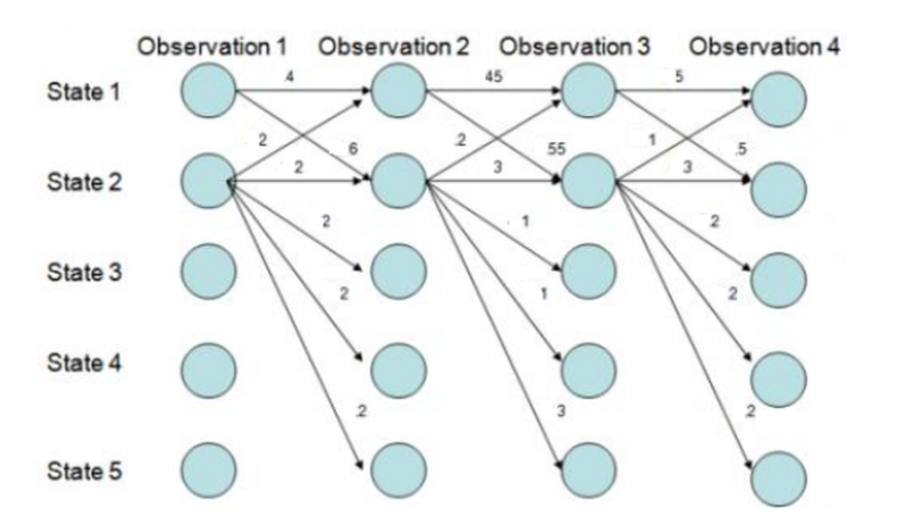
\includegraphics[width=0.5\textwidth]{./1.png}\\
			按道理来说最优的状态转移路径是1->2->2->2,但是MEMM选择的最优状态转换路径为1->1->1->1\\
			2.
			要解决这个问题,可以参考CRF对于标签偏移问题的解决方案来进行处理。MEMM的归一化因子$Z$只是针对了每一个乘子,只是一个局部归一化;但是CRF的归一化因子$Z^\prime$放在了概率函数的最外部,是全局的归一化,数学形式的差别如下:
			\begin{align*}
				P_{MEMM}(\bm{y}|\bm{x}) &= \prod_{i=1}^{n} \frac{exp(\bm{w}^T \bm{f}(y_i,y_{i-1},\bm{x}))}{Z} \\
				P_{CRF}(\bm{y}|\bm{x}) &= \frac{1}{Z^\prime} (exp(\sum_j \sum_{i=1}^{n-1} \lambda_j t_j (y_{i+1},y_i,\bm{x},i) + \sum_k \sum_{i=1}^{n} \mu_k s_k(y_i,\bm{x},i)))
			\end{align*}
			这样一来,CRF可以在每次状态转移之前都会考虑当前状态转移概率在全局中地位,而不是像MEMM只考虑针对单个状态。因此,要解决标签偏移问题,我们可以避免局部归一化,而是进行全局归一化。
		\end{parts}
	\end{solution}
	
\question [40] \textbf{概率图模型进阶}

	本题研究概率图模型里面的变分推断技术。现定义联合分布如下:
	$$p(\mathbf{t}, \boldsymbol{w}, \alpha)=p(\mathbf{t} \mid \boldsymbol{w}) p(\boldsymbol{w} \mid \alpha) p(\alpha)$$
	其中各具体分布为:
	$$p(\mathbf{t} \mid \boldsymbol{w})=\prod_{n=1}^{N} \mathcal{N}\left(t_{n} \mid \boldsymbol{w}^{T} \boldsymbol{\phi}_{n}, \beta^{-1}\right)$$
	$$p(\boldsymbol{w} \mid \alpha)=\mathcal{N}\left(\boldsymbol{w} \mid \mathbf{0}, \alpha^{-1} \boldsymbol{I}\right)$$
	$$p(\alpha)=\operatorname{Gam}\left(\alpha \mid a_{0}, b_{0}\right)=\frac{{b_0}^{a_0} \alpha^{a_0-1} e^{-b_0 \alpha}}{\Gamma(a_0)}$$
	这里,$\mathcal{N}$代表高斯分布,$\operatorname{Gam}\left(\alpha \mid a_{0}, b_{0}\right)$表示变量为$\alpha$,参数为$a_0,b_0$的Gamma分布。
	\begin{parts}
		\part [10] 请使用盘式记法表示联合分布$p(\mathbf{t}, \boldsymbol{w}, \alpha)$。
		
		\part [20] 现在需要寻找对后验概率分布$p(\boldsymbol{w}, \alpha \mid \mathbf{t})$的一个近似。使用变分框架进行分解,得到变分后验概率分布的分解表达式为$q(\boldsymbol{w},\alpha) = q(\boldsymbol{w})q(\alpha)$。首先计算$q^*(\alpha)$,考虑$\alpha$上的概率分布,利用教材公式(14.39),只保留与$\alpha$有函数依赖关系的项,试证明
		$$\ln q^*(\alpha)=\left(a_{0}-1\right) \ln \alpha-b_{0} \alpha+\frac{M}{2} \ln \alpha-\frac{\alpha}{2} \mathbb{E}\left[\boldsymbol{w}^{T} \boldsymbol{w}\right]+\text { 常数 }$$
		这里$M$表示与$\boldsymbol{w}$和$\alpha$无关的常数。
		
		\part [10] 由上一题得到的结果,观察发现这是Gamma分布的对数,因此$q^*(\alpha)$仍然服从如下Gamma分布
		$$q^{*}(\alpha)=\operatorname{Gam}\left(\alpha \mid a_{N}, b_{N}\right)$$
		问:(a)计算$a_{N}, b_{N}$的具体值(提示:由上一题计算Gamma分布对数$\ln p(\alpha)$的结果观察$\alpha$和$\ln\alpha$的系数便可简单解决)
		(b)比较$q^{*}(\alpha)$与$p(\alpha)$的相似度,总结变分推断的效果。(简单作答即可)
	\end{parts}
	
	
	
	\begin{solution}
		\begin{parts}
			\part 
			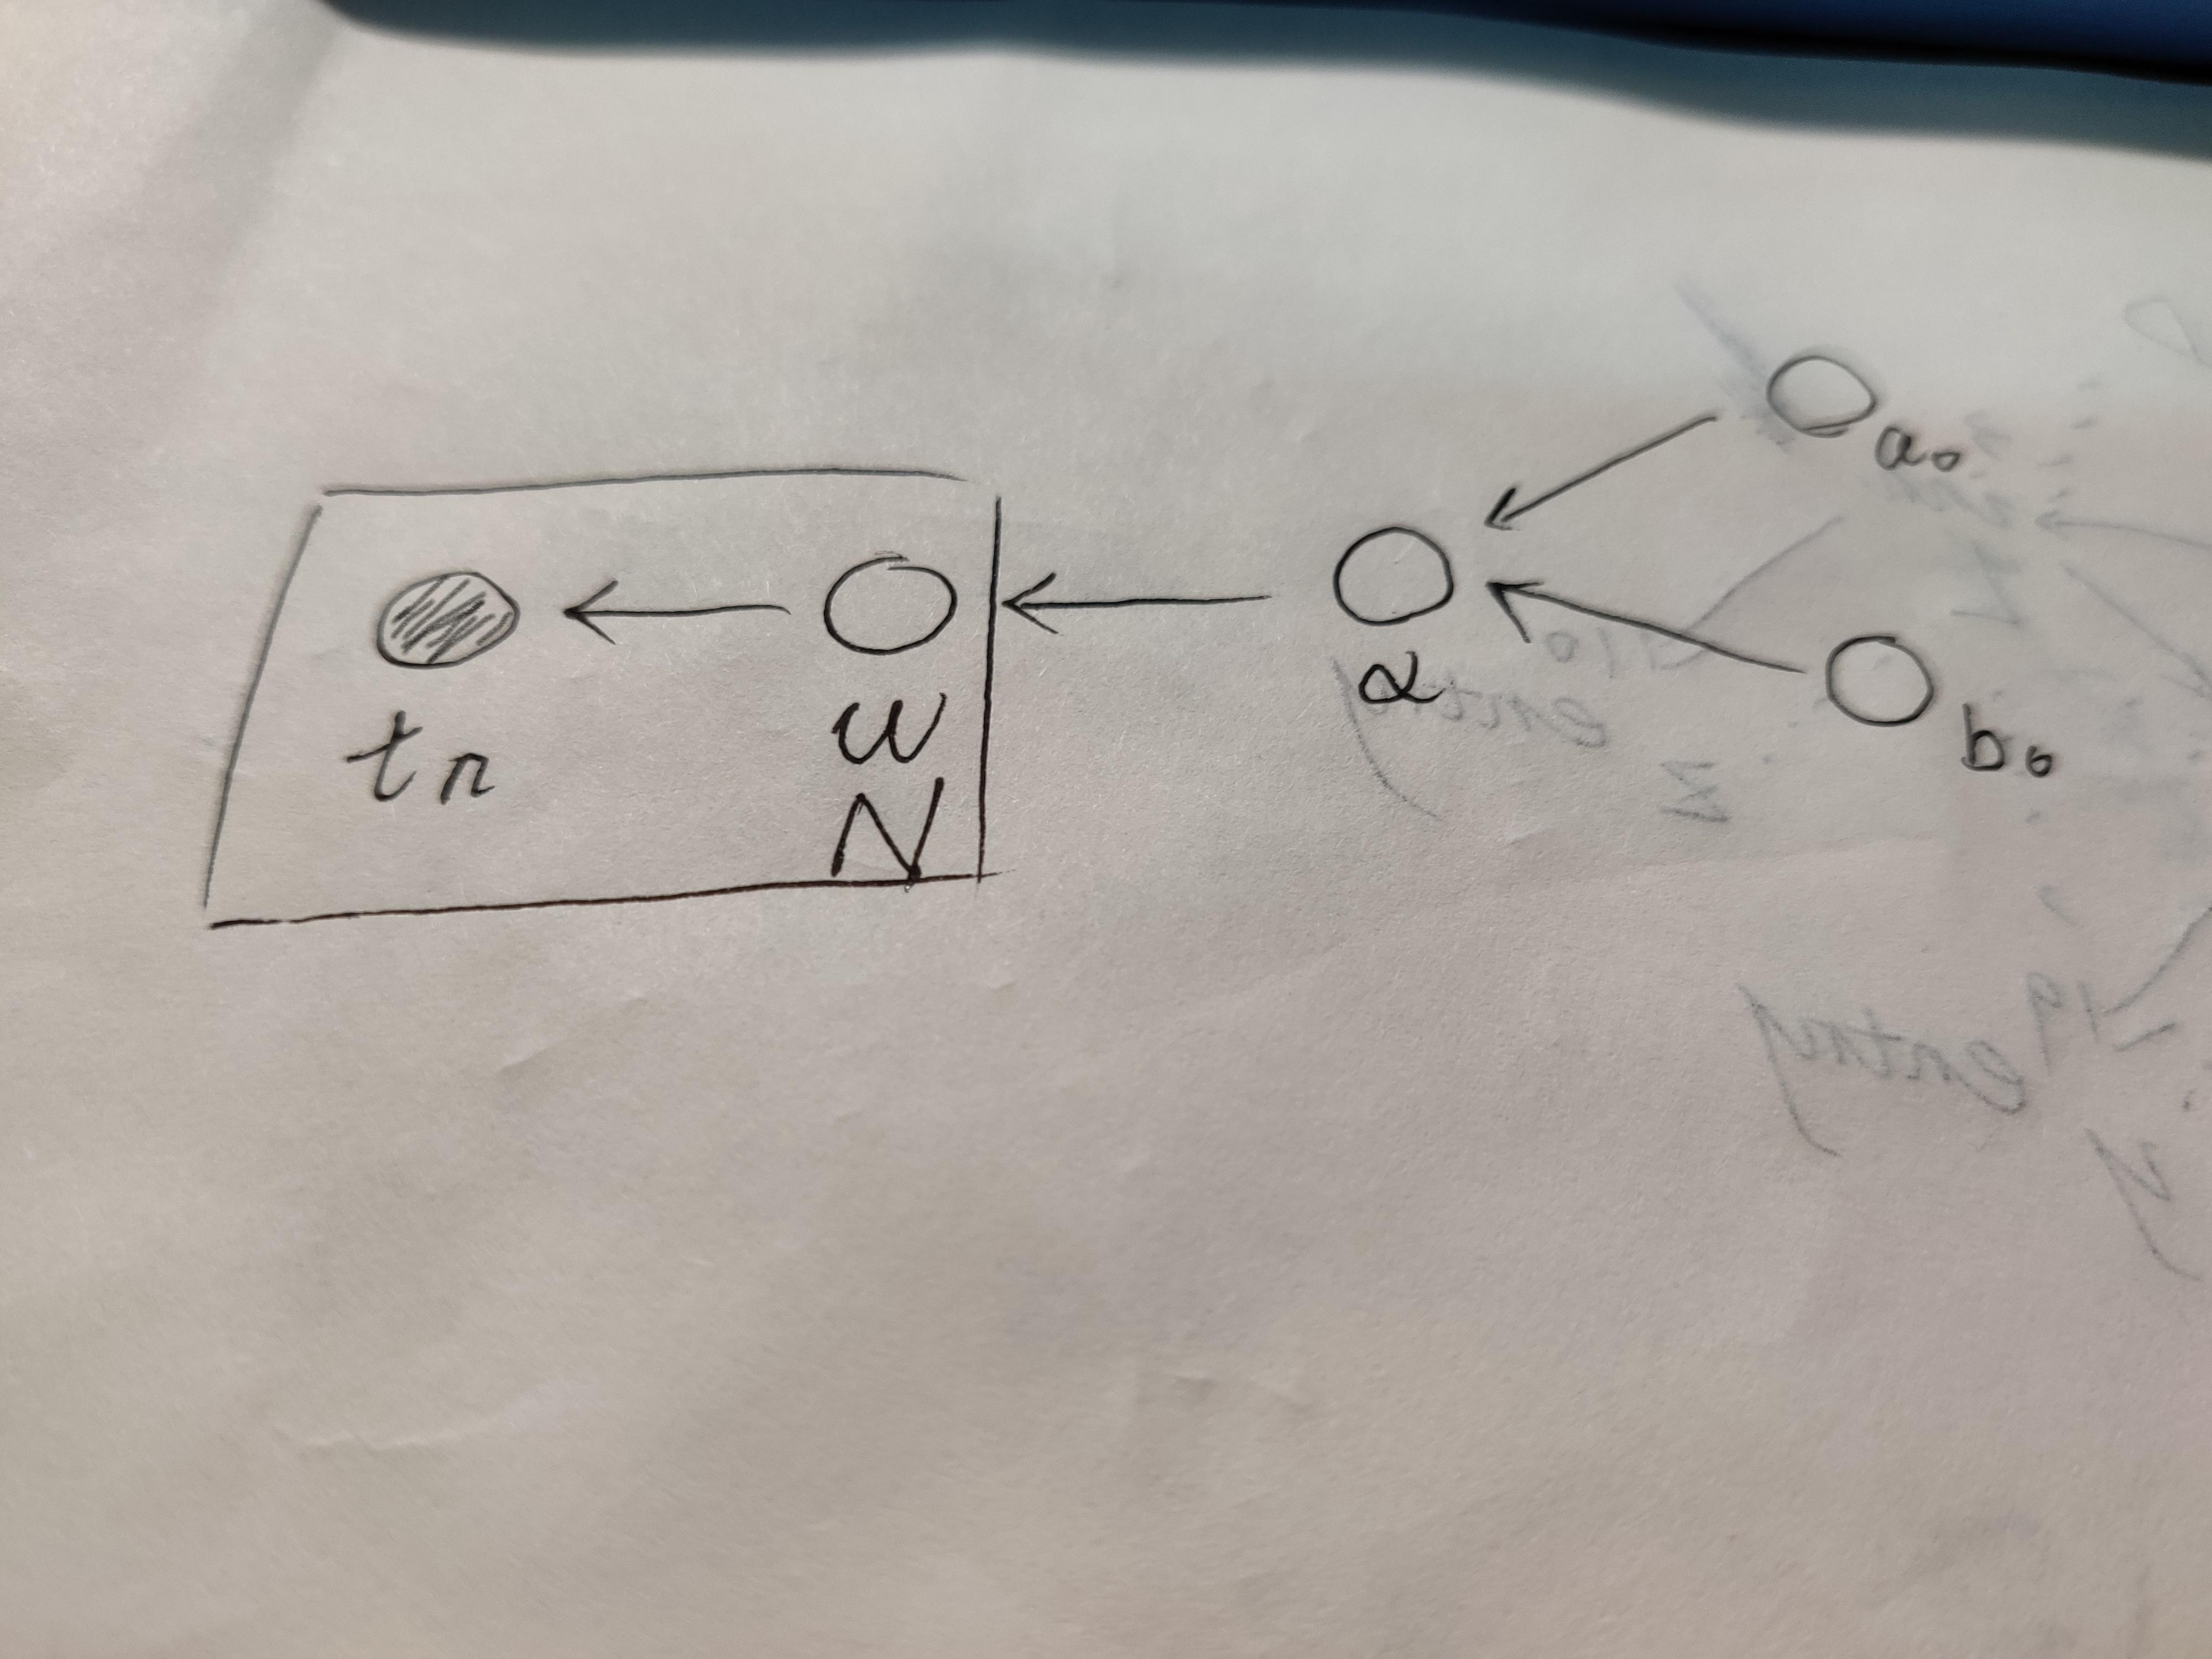
\includegraphics[width=0.5\textwidth]{./Inked2.jpg}\\
			\part
			\begin{align*}
				\ln q^*(\alpha) &= \mathbb{E}[\ln p(\bm{t},\bm{w},\alpha)] + const\\
								&= \ln p(\bm{t}|\bm{w}) + \ln p(\bm{w}|\alpha) + \ln p(\alpha) \\
								&= \mathbb{E}[-\frac{1}{2} \bm{w}^T \alpha \bm{w} - \ln(2\pi^{\frac{d_1}{2}}) - \frac{1}{2} \ln \alpha
								+ a_0 \ln b_0 + (a_0 -1 )\ln \alpha - b_0 \alpha \\
								&- \ln (\Gamma(a_0)) +  \ln p(\bm{t}|\bm{w})] + const
			\end{align*}
			因为只保留与$\alpha$有函数依赖关系的项,因此可以化成
			\begin{align*}
				\ln q^*(\alpha) &= \mathbb{E}[-\frac{\alpha}{2} \bm{w}^T  \bm{w} - \frac{1}{2} \ln \alpha + (a_0 -1 )\ln \alpha - b_0 \alpha] + const \\
								&= -\frac{\alpha}{2}\mathbb{E}[\bm{w}^T  \bm{w}] + (a_0 -1 )\ln \alpha - b_0 \alpha - \frac{1}{2} \ln \alpha + const
			\end{align*}
			得证.
			\part
			(a) 
			\begin{align*}
				a_N - 1 &= a_0 - 1 + \frac{M}{2} \\
				-b_N &= -b_0 - \frac{\mathbb{E}[\bm{w}^T  \bm{w}]}{2}\\
				a_N &= a_0 + \frac{M}{2} \\
				b_N &= b_0 + \frac{\mathbb{E}[\bm{w}^T  \bm{w}]}{2}
			\end{align*}
			根据上题解出$M=-1$,
			\begin{align*}
				a_N &= a_0 - \frac{1}{2} \\
				b_N &= b_0 + \frac{\mathbb{E}[\bm{w}^T  \bm{w}]}{2}
			\end{align*}
			(b) 
			1.
			$q^*(\alpha)$与$p(\alpha)$同为$Gamma$分布,且仅仅在参数$a_i,b_i$上有常数级别的差距,可以基本认为这两者的相似度很高。\\
			2.
			我们原始目标在于根据已有观测到的数据去推断分布$p$,但是因为隐变量$z$的存在以及其他因素的影响,我们难以高效地直接求解分布$p$。通过变分推断,我们可以寻找一个容易表达并且容易求解的近似分布$q$,在$q$分布与$p$分布差距很小的情况下,我们就可以认为这个近似关系是成立的,就可以将$q$分布作为我们的推断结果。简单来说,变分推断将原本需要大量时间开销的计算归结为求解evidence lower bound的优化问题:
			\begin{align*}
				\arg \max ELBO(q) \\
				and ELBO(q) &= E[\log p(\bm{z},\bm{x})] -  E[\log q(\bm{z})] \\
						&= E[\log p(\bm{z})] + E[\log p(\bm{x}|\bm{z})] -  E[\log q(\bm{z})] \\
						&= E[\log p(\bm{x}|\bm{z})] - KL(q(\bm{z})||p(\bm{z})) 
			\end{align*}
			之后,我们利用平均场假设等假设条件
			\begin{align*}
				q(\bm{z}) = \prod_{i=1}^{M} q_i(\bm{z_i})
			\end{align*}
			去化简我们所要求解的优化问题,并得知变量子集$\bm{z}_j$服从的最优分布$q_j^*$满足
			\begin{align*}
				\ln q_j^*(\bm{z}_j) = \mathbb{E}_{i\not=j}[\ln p(\bm{x},\bm{z})] + const
			\end{align*}
			借助这个式子,我们就可以在恰当地分割独立变量子集$\bm{z}_j$并选择$q_i$所服从的分布的基础上,高效地对隐变量$\bm{z}$进行推断,从而得出近似分布。
		\end{parts}
	\end{solution}
	
\end{questions}


\end{document}